\documentclass[convert = false, tikz]{standalone}
\usepackage[utf8]{inputenc}
\usepackage{tikz}
\usetikzlibrary{automata, positioning, arrows}
 
\usepackage{../../../../style_automata}

% arara: pdflatex
% arara: latexmk: { clean: partial }

\begin{document}
    \tikzset{
    greenText/.style={text=red},
    greenNode/.style={greenText, draw=red}
    }
    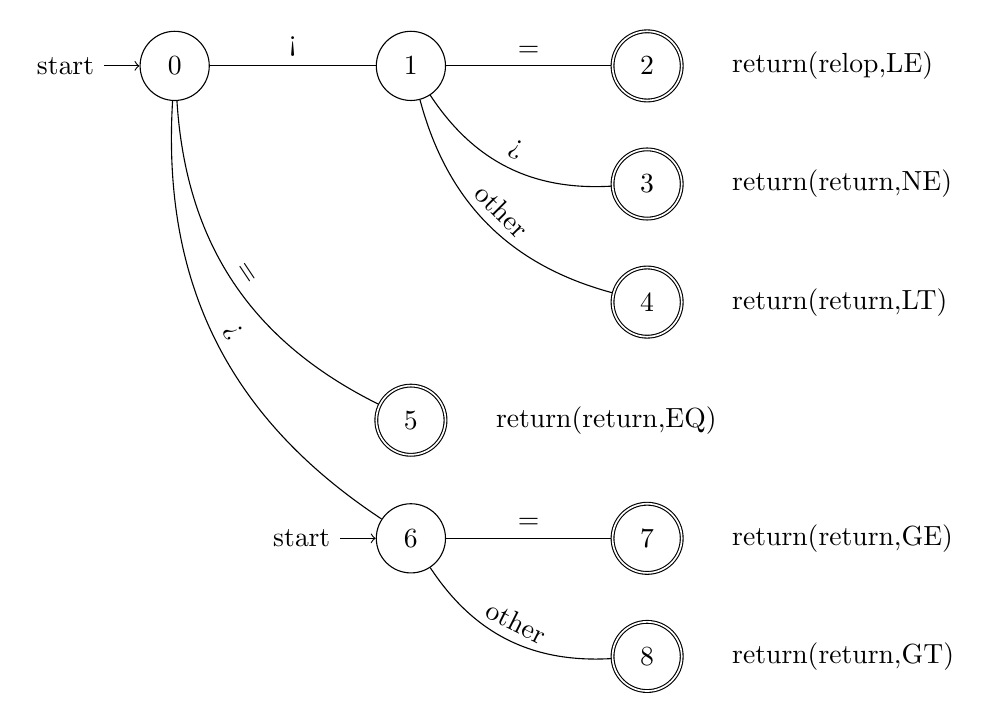
\begin{tikzpicture}[x=3cm, y=1.5cm]
        % Draw grid with help lines
        %\draw[help lines,step=5mm,gray!20] (-1,-1) grid (3,6);
        \begin{scope}[]
        
        % start node
        \node (0) [state, initial] at (0,5) {0};

        % first branch
        \node (1) [state] at (1,5) {1};
        \node (2) [state, accepting] at (2,5) {2};
        \node (3) [state, accepting] at (2,4) {3};
        \node (4) [state, accepting] at (2,3) {4};

        % second branch
        \node (5) [state, accepting] at (1,2) {5};

        % third branch
        \node (6) [state, initial] at (1,1) {6};
        \node (7) [state, accepting] at (2,1) {7};
        \node (8) [state, accepting] at (2,0) {8};

        \draw (0) -- node[above,sloped] {<} (1);
        \draw (1) -- node[above,sloped] {=} (2);
        \draw (1) to[bend right] node[above,sloped] {>} (3);
        \draw (1) to[bend right] node[above,sloped] {other} (4);
        \draw (0) to[bend right] node[above,sloped] {=} (5);
        \draw (0) to[bend right] node[above,sloped] {>} (6);
        \draw (6) -- node[above,sloped] {=} (7);
        \draw (6) to[bend right] node[above,sloped] {other} (8);

        % return text
        \node[right=0.5cm of 2] {return(relop,LE)};
        \node[right=0.5cm of 3] {return(return,NE)};
        \node[right=0.5cm of 4] {return(return,LT)};
        \node[right=0.5cm of 5] {return(return,EQ)};
        \node[right=0.5cm of 7] {return(return,GE)};
        \node[right=0.5cm of 8] {return(return,GT)};

        \end{scope}
    \end{tikzpicture}
\end{document}
